\documentclass{standalone}
\usepackage{tikz}
\usepackage{ctex,siunitx}
\setCJKmainfont{Noto Serif CJK SC}
\usepackage{tkz-euclide}
\usepackage{amsmath}
\usetikzlibrary{patterns, calc,3d}
\usetikzlibrary {decorations.pathmorphing,decorations.pathreplacing,decorations.shapes}
\begin{document}
\small
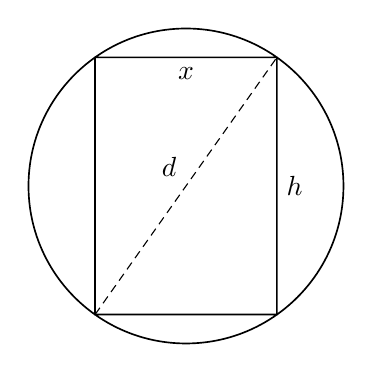
\begin{tikzpicture}[>=latex,scale=1.0]
  \draw[semithick](0,0)circle(2)({-2*sqrt(3)/3},{-2*sqrt(6)/3})rectangle({2*sqrt(3)/3},{2*sqrt(6)/3});
  \draw[densely dashed]({-2*sqrt(3)/3},{-2*sqrt(6)/3})--({2*sqrt(3)/3},{2*sqrt(6)/3})node[midway,above left]{$d$};
  \node at ({2*sqrt(3)/3},0)[right]{$h$};
  \node at (0,{2*sqrt(6)/3})[below]{$x$};
\end{tikzpicture}
\end{document}